\tikzset{every picture/.style={line width=0.75pt}} %set default line width to 0.75pt        

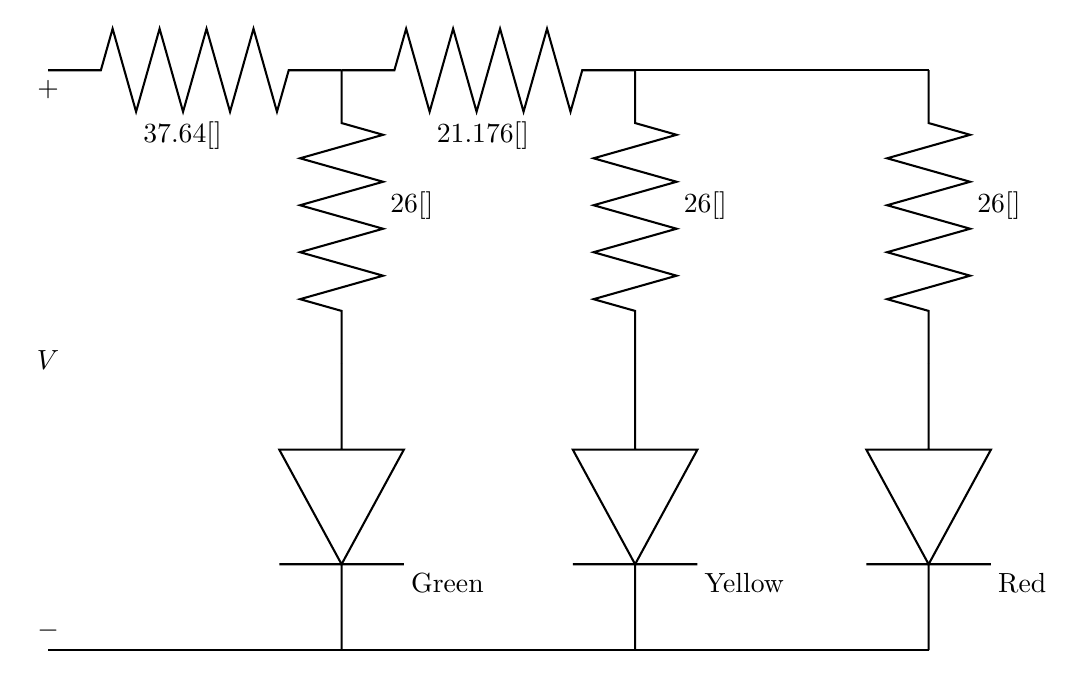
\begin{tikzpicture}[x=0.75pt,y=0.75pt,yscale=-1,xscale=1]
%uncomment if require: \path (0,757); %set diagram left start at 0, and has height of 757

%Shape: Diode [id:dp9916766022166023] 
\draw   (567,293.4) -- (537,348.6) -- (507,293.4) -- (567,293.4) -- cycle (537,252) -- (537,293.4) (567,348.6) -- (507,348.6) (537,348.6) -- (537,390) ;
%Shape: Diode [id:dp47724199606317685] 
\draw   (425.58,293.4) -- (395.58,348.6) -- (365.58,293.4) -- (425.58,293.4) -- cycle (395.58,252) -- (395.58,293.4) (425.58,348.6) -- (365.58,348.6) (395.58,348.6) -- (395.58,390) ;
%Straight Lines [id:da43394379079125567] 
\draw    (537,390) -- (395.58,390) ;
%Shape: Resistor [id:dp7260924477087448] 
\draw   (537,110.58) -- (537,136.03) -- (557,141.69) -- (517,153.01) -- (557,164.32) -- (517,175.63) -- (557,186.95) -- (517,198.26) -- (557,209.57) -- (517,220.89) -- (537,226.54) -- (537,252) ;
%Shape: Resistor [id:dp09973725738727013] 
\draw   (395.58,110.58) -- (395.58,136.03) -- (415.58,141.69) -- (375.58,153.01) -- (415.58,164.32) -- (375.58,175.63) -- (415.58,186.95) -- (375.58,198.26) -- (415.58,209.57) -- (375.58,220.89) -- (395.58,226.54) -- (395.58,252) ;
%Straight Lines [id:da9934104451259984] 
\draw    (537,110.58) -- (395.58,110.58) ;
%Shape: Resistor [id:dp5223648498783691] 
\draw   (254.16,110.58) -- (279.61,110.58) -- (285.27,90.58) -- (296.58,130.58) -- (307.9,90.58) -- (319.21,130.58) -- (330.52,90.58) -- (341.84,130.58) -- (353.15,90.58) -- (364.47,130.58) -- (370.12,110.58) -- (395.58,110.58) ;
%Shape: Diode [id:dp30609907031657446] 
\draw   (284.16,293.4) -- (254.16,348.6) -- (224.16,293.4) -- (284.16,293.4) -- cycle (254.16,252) -- (254.16,293.4) (284.16,348.6) -- (224.16,348.6) (254.16,348.6) -- (254.16,390) ;
%Shape: Resistor [id:dp3336013122238709] 
\draw   (254.16,110.58) -- (254.16,136.03) -- (274.16,141.69) -- (234.16,153.01) -- (274.16,164.32) -- (234.16,175.63) -- (274.16,186.95) -- (234.16,198.26) -- (274.16,209.57) -- (234.16,220.89) -- (254.16,226.54) -- (254.16,252) ;
%Straight Lines [id:da4142874846716025] 
\draw    (395.58,390) -- (254.16,390) ;
%Shape: Resistor [id:dp416533824669727] 
\draw   (112.74,110.58) -- (138.19,110.58) -- (143.85,90.58) -- (155.16,130.58) -- (166.48,90.58) -- (177.79,130.58) -- (189.1,90.58) -- (200.42,130.58) -- (211.73,90.58) -- (223.04,130.58) -- (228.7,110.58) -- (254.16,110.58) ;
%Straight Lines [id:da6359356780714503] 
\draw    (254.16,390) -- (112.74,390) ;

% Text Node
\draw (559,167.72) node [anchor=north west][inner sep=0.75pt]    {$26[ \si{\ohm}]$};
% Text Node
\draw (417.58,167.72) node [anchor=north west][inner sep=0.75pt]    {$26[ \si{\ohm}]$};
% Text Node
\draw (276.16,167.72) node [anchor=north west][inner sep=0.75pt]    {$26[ \si{\ohm}]$};
% Text Node
\draw (298.58,133.98) node [anchor=north west][inner sep=0.75pt]    {$21.176[ \si{\ohm}]$};
% Text Node
\draw (157.16,133.98) node [anchor=north west][inner sep=0.75pt]    {$37.64[ \si{\ohm}]$};
% Text Node
\draw (569,351.6) node [anchor=north west][inner sep=0.75pt]   [align=left] {Red};
% Text Node
\draw (427.58,351.6) node [anchor=north west][inner sep=0.75pt]   [align=left] {Yellow};
% Text Node
\draw (286.16,351.6) node [anchor=north west][inner sep=0.75pt]   [align=left] {Green};
% Text Node
\draw (112.74,113.98) node [anchor=north] [inner sep=0.75pt]    {$+$};
% Text Node
\draw (112.74,386.6) node [anchor=south] [inner sep=0.75pt]    {$-$};
% Text Node
\draw (112.74,250.29) node    {$V$};


\end{tikzpicture}
